\chapter{Komposition}

Sind die beiden Bilder erst einmal fertig verzerrt worden, so werden
sie nun, wie eingangs beschrieben, durch eine Kreuzblende 
zusammengefuegt. Zu beachten ist, dass das Zielbild
in Richtung des Quellbildes gewarpt wurde. Die Bildsequenzen
fuer die beiden Bilder sehen dementsprechend folgendermassen
aus:

\begin{figure}[htbp]
	\centering


	
	\begin{subfigure}[b]{0.19\textwidth}
		\centering
		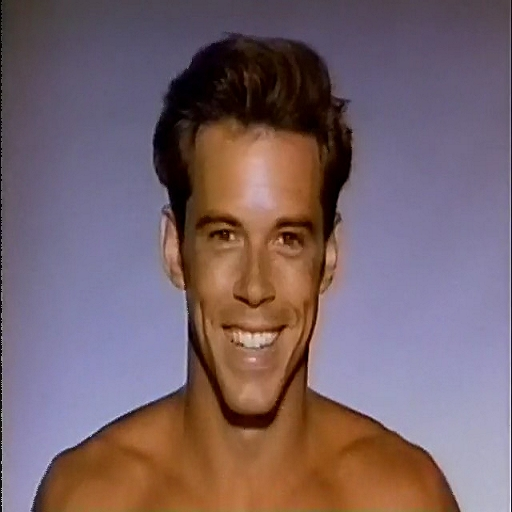
\includegraphics[width=\textwidth]{source/src0.jpg} % Replace 'image1' with your image file name
		\caption{}
	\end{subfigure}
		\begin{subfigure}[b]{0.19\textwidth}
		\centering
		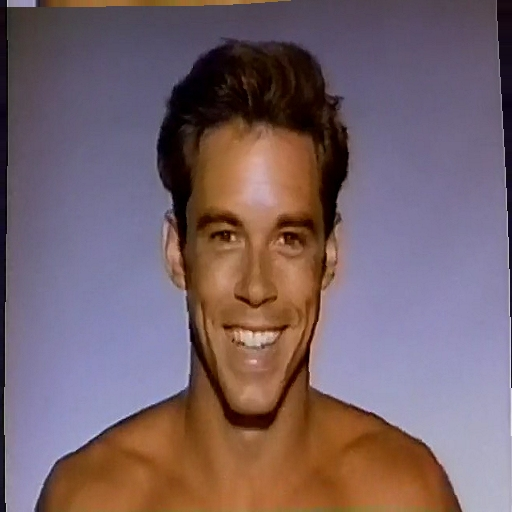
\includegraphics[width=\textwidth]{source/src1.jpg} % Replace 'image1' with your image file name
		\caption{}
	\end{subfigure}
		\begin{subfigure}[b]{0.19\textwidth}
		\centering
		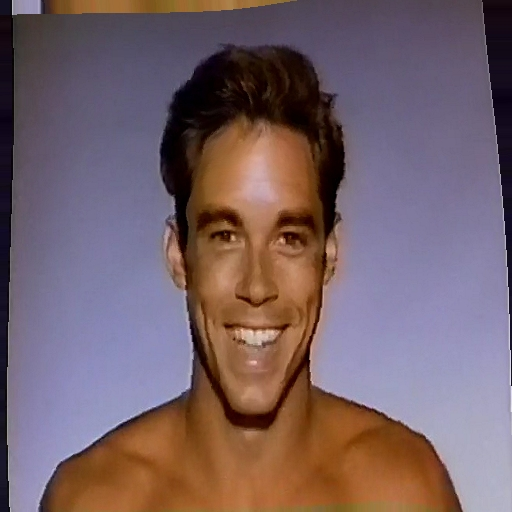
\includegraphics[width=\textwidth]{source/src2.jpg} % Replace 'image1' with your image file name
		\caption{}
	\end{subfigure}
		\begin{subfigure}[b]{0.19\textwidth}
		\centering
		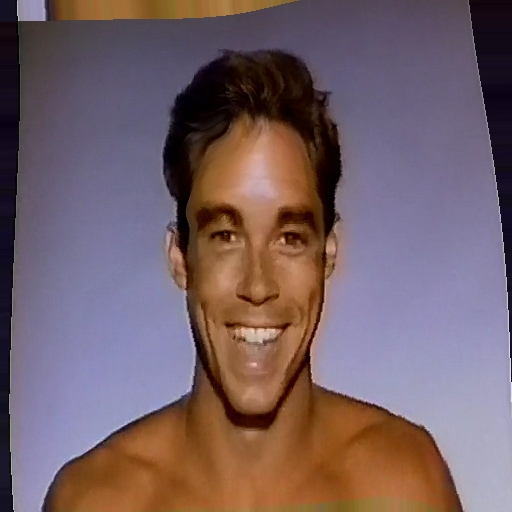
\includegraphics[width=\textwidth]{source/src3.jpg} % Replace 'image1' with your image file name
		\caption{}
	\end{subfigure}
		\begin{subfigure}[b]{0.19\textwidth}
		\centering
		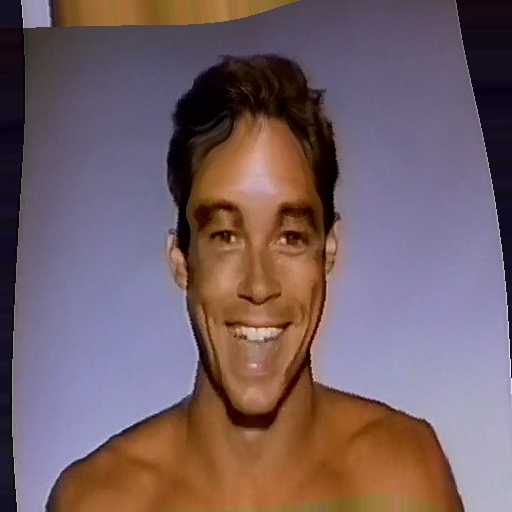
\includegraphics[width=\textwidth]{source/src4.jpg} % Replace 'image1' with your image file name
		\caption{}
	\end{subfigure}
		\begin{subfigure}[b]{0.19\textwidth}
		\centering
		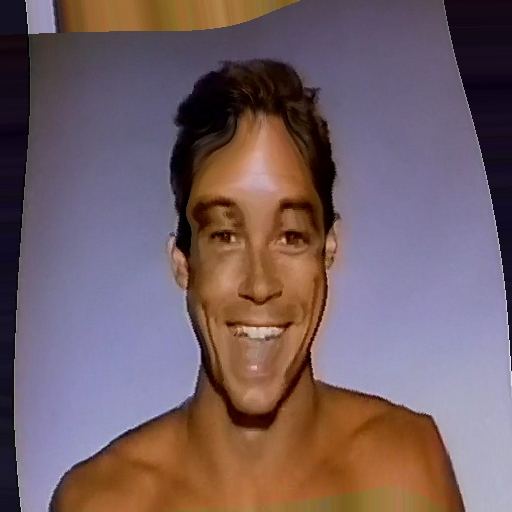
\includegraphics[width=\textwidth]{source/src5.jpg} % Replace 'image1' with your image file name
		\caption{}
	\end{subfigure}
			\begin{subfigure}[b]{0.19\textwidth}
		\centering
		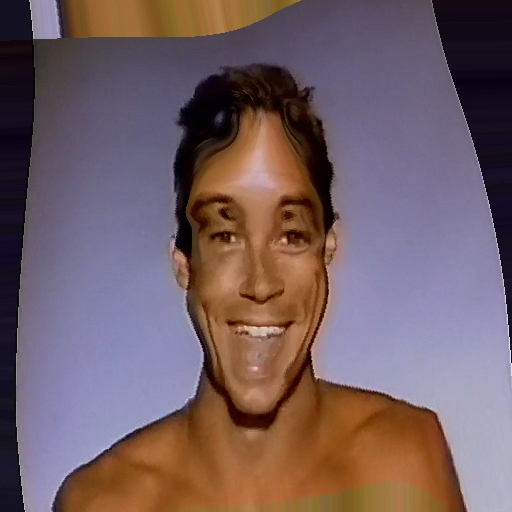
\includegraphics[width=\textwidth]{source/src6.jpg} % Replace 'image1' with your image file name
		\caption{}
	\end{subfigure}
	

	
		\caption{Quell- zu Ziel warps}
	\label{fig:sources}
	\end{figure}
	% Repeat the subfigure environment for each image
	% ... (Add more subfigures for the remaining images)
	
	% Example of a second row
\begin{figure}[htbp]
	\centering

	    	
	\begin{subfigure}[b]{0.19\textwidth}
		\centering
		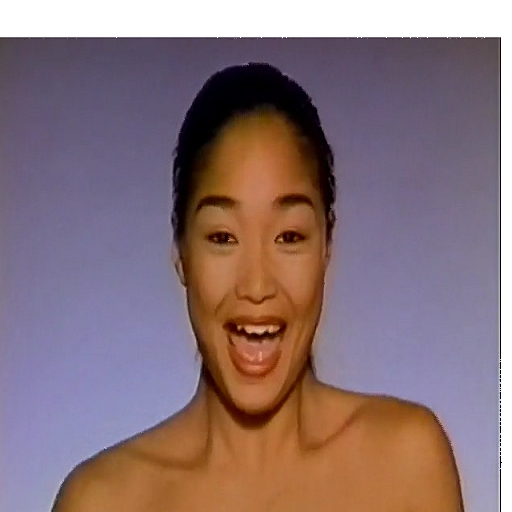
\includegraphics[width=\textwidth]{dst/dest6} % Replace 'image7' with your image file name
		\caption{}
	\end{subfigure}
		\begin{subfigure}[b]{0.19\textwidth}
		\centering
		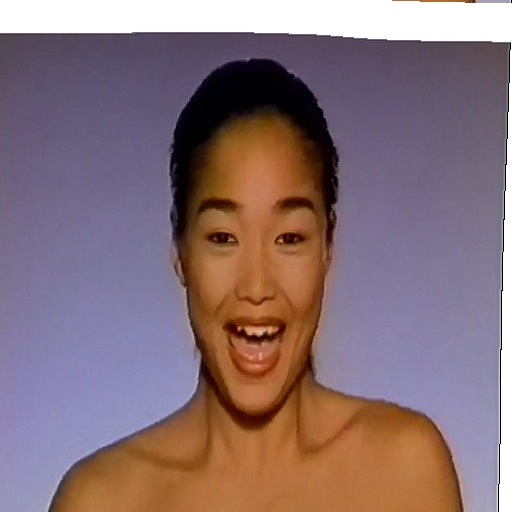
\includegraphics[width=\textwidth]{dst/dest5} % Replace 'image7' with your image file name
		\caption{}
	\end{subfigure}
		\begin{subfigure}[b]{0.19\textwidth}
		\centering
		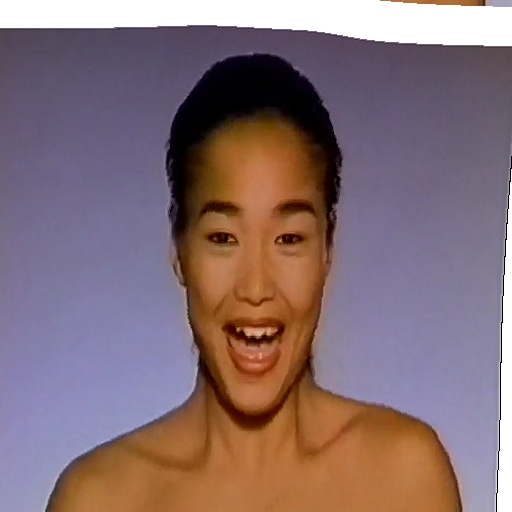
\includegraphics[width=\textwidth]{dst/dest4} % Replace 'image7' with your image file name
		\caption{}
	\end{subfigure}
		\begin{subfigure}[b]{0.19\textwidth}
		\centering
		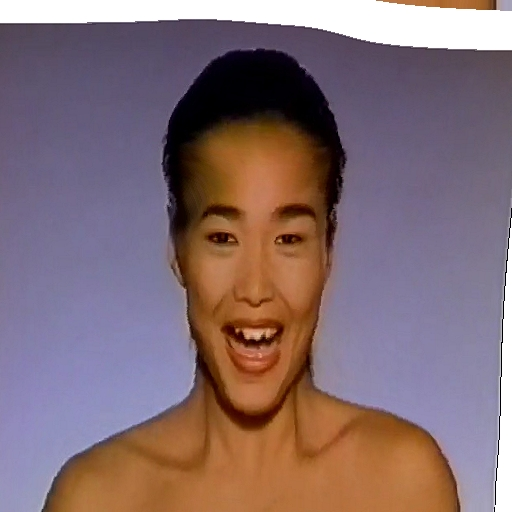
\includegraphics[width=\textwidth]{dst/dest3} % Replace 'image7' with your image file name
		\caption{}
	\end{subfigure}
		\begin{subfigure}[b]{0.19\textwidth}
		\centering
		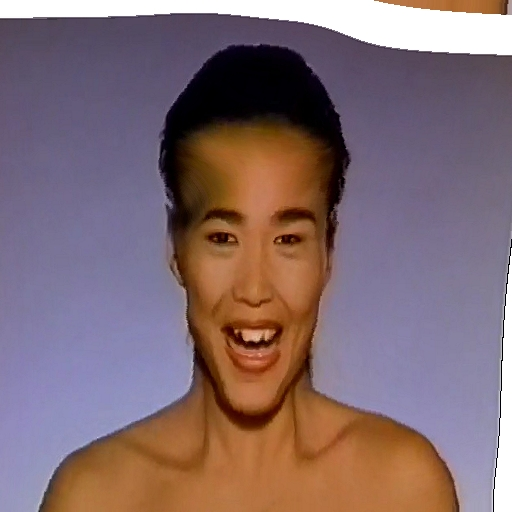
\includegraphics[width=\textwidth]{dst/dest2} % Replace 'image7' with your image file name
		\caption{}
	\end{subfigure}
		\begin{subfigure}[b]{0.19\textwidth}
		\centering
		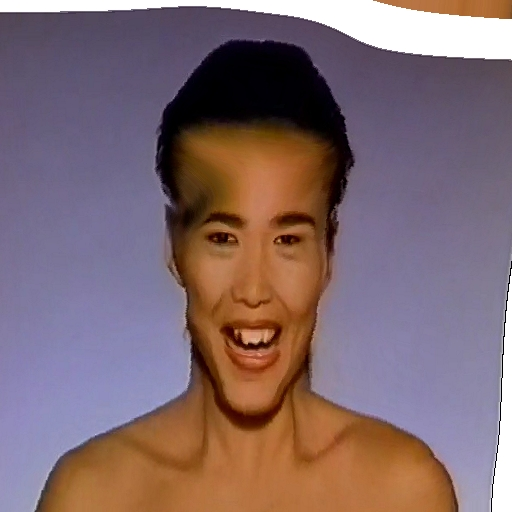
\includegraphics[width=\textwidth]{dst/dest1} % Replace 'image7' with your image file name
		\caption{}
	\end{subfigure}
		\begin{subfigure}[b]{0.19\textwidth}
		\centering
		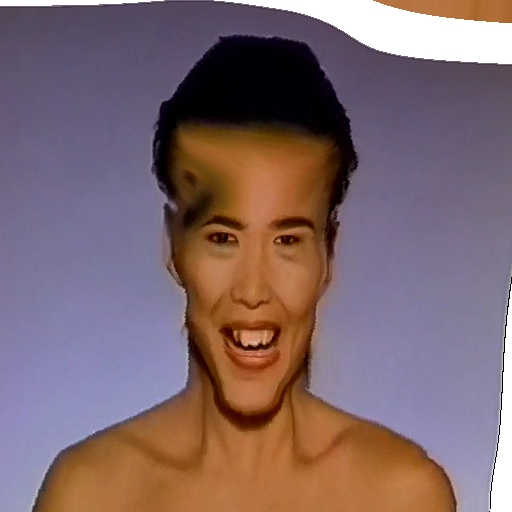
\includegraphics[width=\textwidth]{dst/dest0} % Replace 'image7' with your image file name
		\caption{}
	\end{subfigure}
	% ... (Add subfigures for the second row)
	
		    
	\caption{Ziel- zu Quell warps}
	\label{fig:destinations}
\end{figure}

Die Sequenz in Abbildung \ref{fig:destinations} muss zunaechst noch
in ihrer Reihenfolge geaendert werden bevor
die Kreuzblende angewendet wird.

\begin{figure}[htbp]
	\centering

		    	
	\begin{subfigure}[b]{0.4\textwidth}
		\centering
		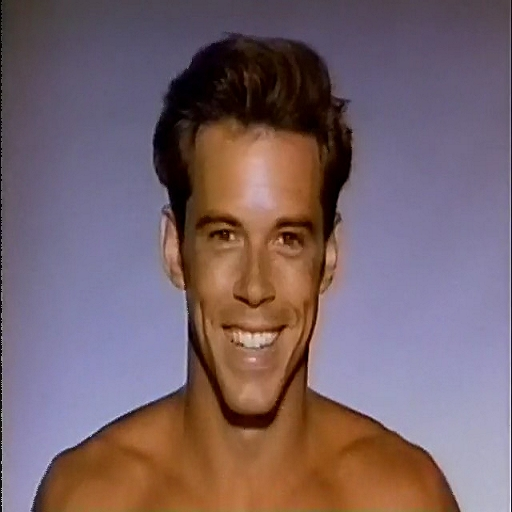
\includegraphics[width=\textwidth]{final/final0} % Replace 'image7' with your image file name
		\caption{}
	\end{subfigure}
	\begin{subfigure}[b]{0.4\textwidth}
		\centering
		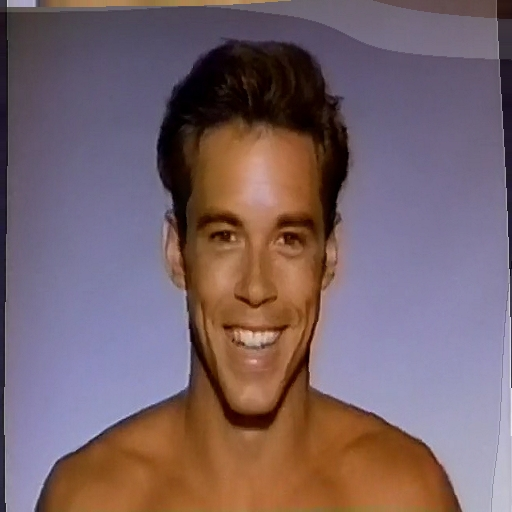
\includegraphics[width=\textwidth]{final/final1} % Replace 'image7' with your image file name
		\caption{}
	\end{subfigure}
	\begin{subfigure}[b]{0.4\textwidth}
		\centering
		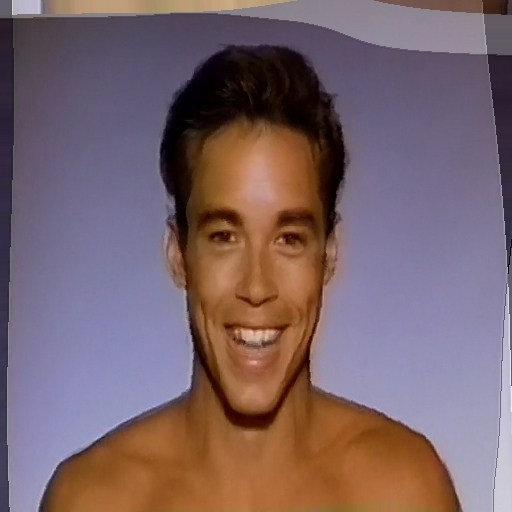
\includegraphics[width=\textwidth]{final/final2} % Replace 'image7' with your image file name
		\caption{}
	\end{subfigure}
	\begin{subfigure}[b]{0.4\textwidth}
		\centering
		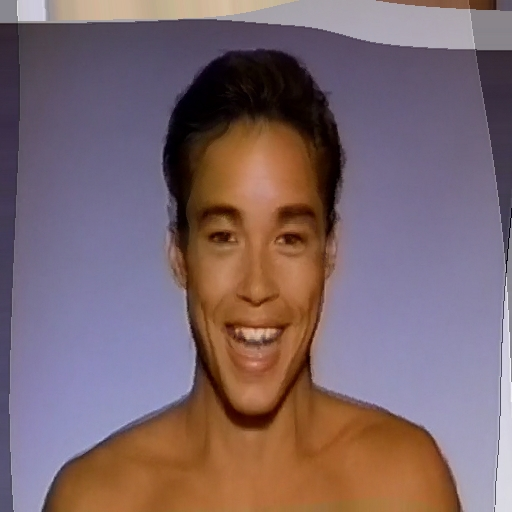
\includegraphics[width=\textwidth]{final/final3} % Replace 'image7' with your image file name
		\caption{}
	\end{subfigure}
	\begin{subfigure}[b]{0.4\textwidth}
		\centering
		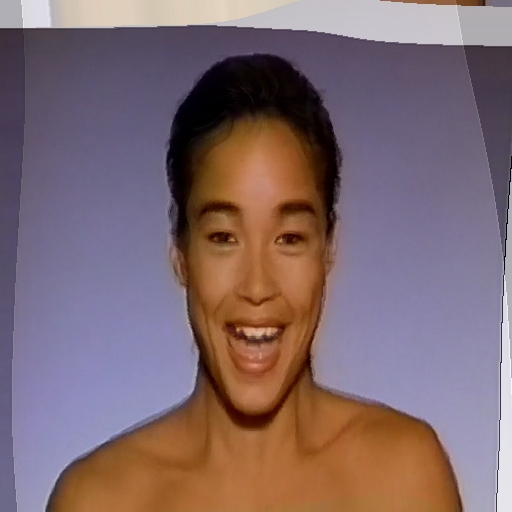
\includegraphics[width=\textwidth]{final/final4} % Replace 'image7' with your image file name
		\caption{}
	\end{subfigure}
	\begin{subfigure}[b]{0.4\textwidth}
		\centering
		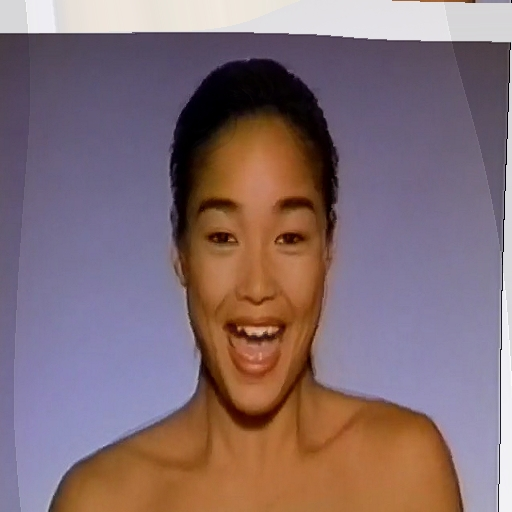
\includegraphics[width=\textwidth]{final/final5} % Replace 'image7' with your image file name
		\caption{}
	\end{subfigure}
	\begin{subfigure}[b]{0.4\textwidth}
		\centering
		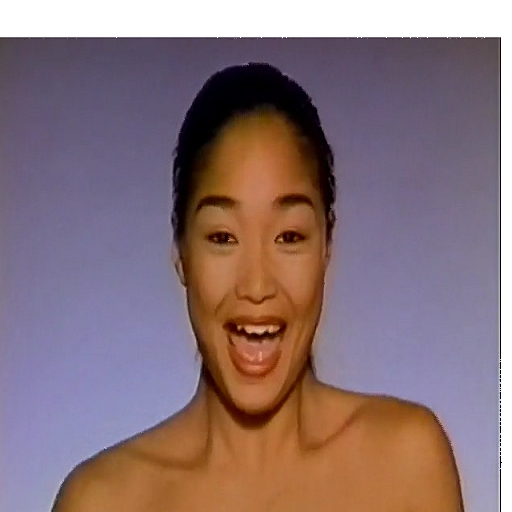
\includegraphics[width=\textwidth]{final/final6} % Replace 'image7' with your image file name
		\caption{}
	\end{subfigure}
	% ... (Add subfigures for the second row)
			    
	\caption{Finale Komposition}
	\label{fig:final}
\end{figure}


